\documentclass[xcolor={usenames,svgnames,x11names,dvipsnames,table}]{beamer}

\usetheme{SBUclass}

\usepackage{mypackages}

\title{\texorpdfstring{Language \& Technology}{Language and Technology}}
\subtitle{Lecture 1: What is Language Technology?}
\author{Al{\"e}na Aks{\"e}nova \& Aniello De Santo}
\institute{Stony Brook University\\\texttt{alena.aksenova@stonybrook.edu}\\\texttt{aniello.desanto@stonybrook.edu}}
\date{}


\begin{document}
\unnumbered{
\begin{frame}
	\titlepage
\end{frame}
}

\begin{frame}[t]{Why Language Technology?}
    \begin{columns}
        \column{.6\linewidth}

        Because language is important!
        \begin{itemize}
            \item communication system\\
                \subpoint{transfer message, convey information}
            \item cultural artefact\\
                \subpoint{signal group membership\\
                    (dialects, sociolects)}
            \item uniquely human cognitive ability\\
                \subpoint{language in the brain}
        \end{itemize}

        \column[t]{.3\linewidth}
        \centering
        \visible<2->{
\includegraphics[height=10em]{./img/homosapiens}}

        \only<3>{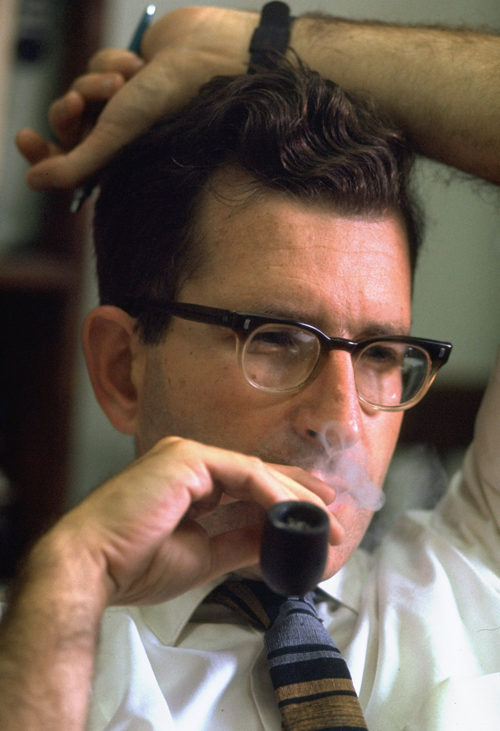
\includegraphics[height=10em]{./img/chomsky_young}}

        \only<4>{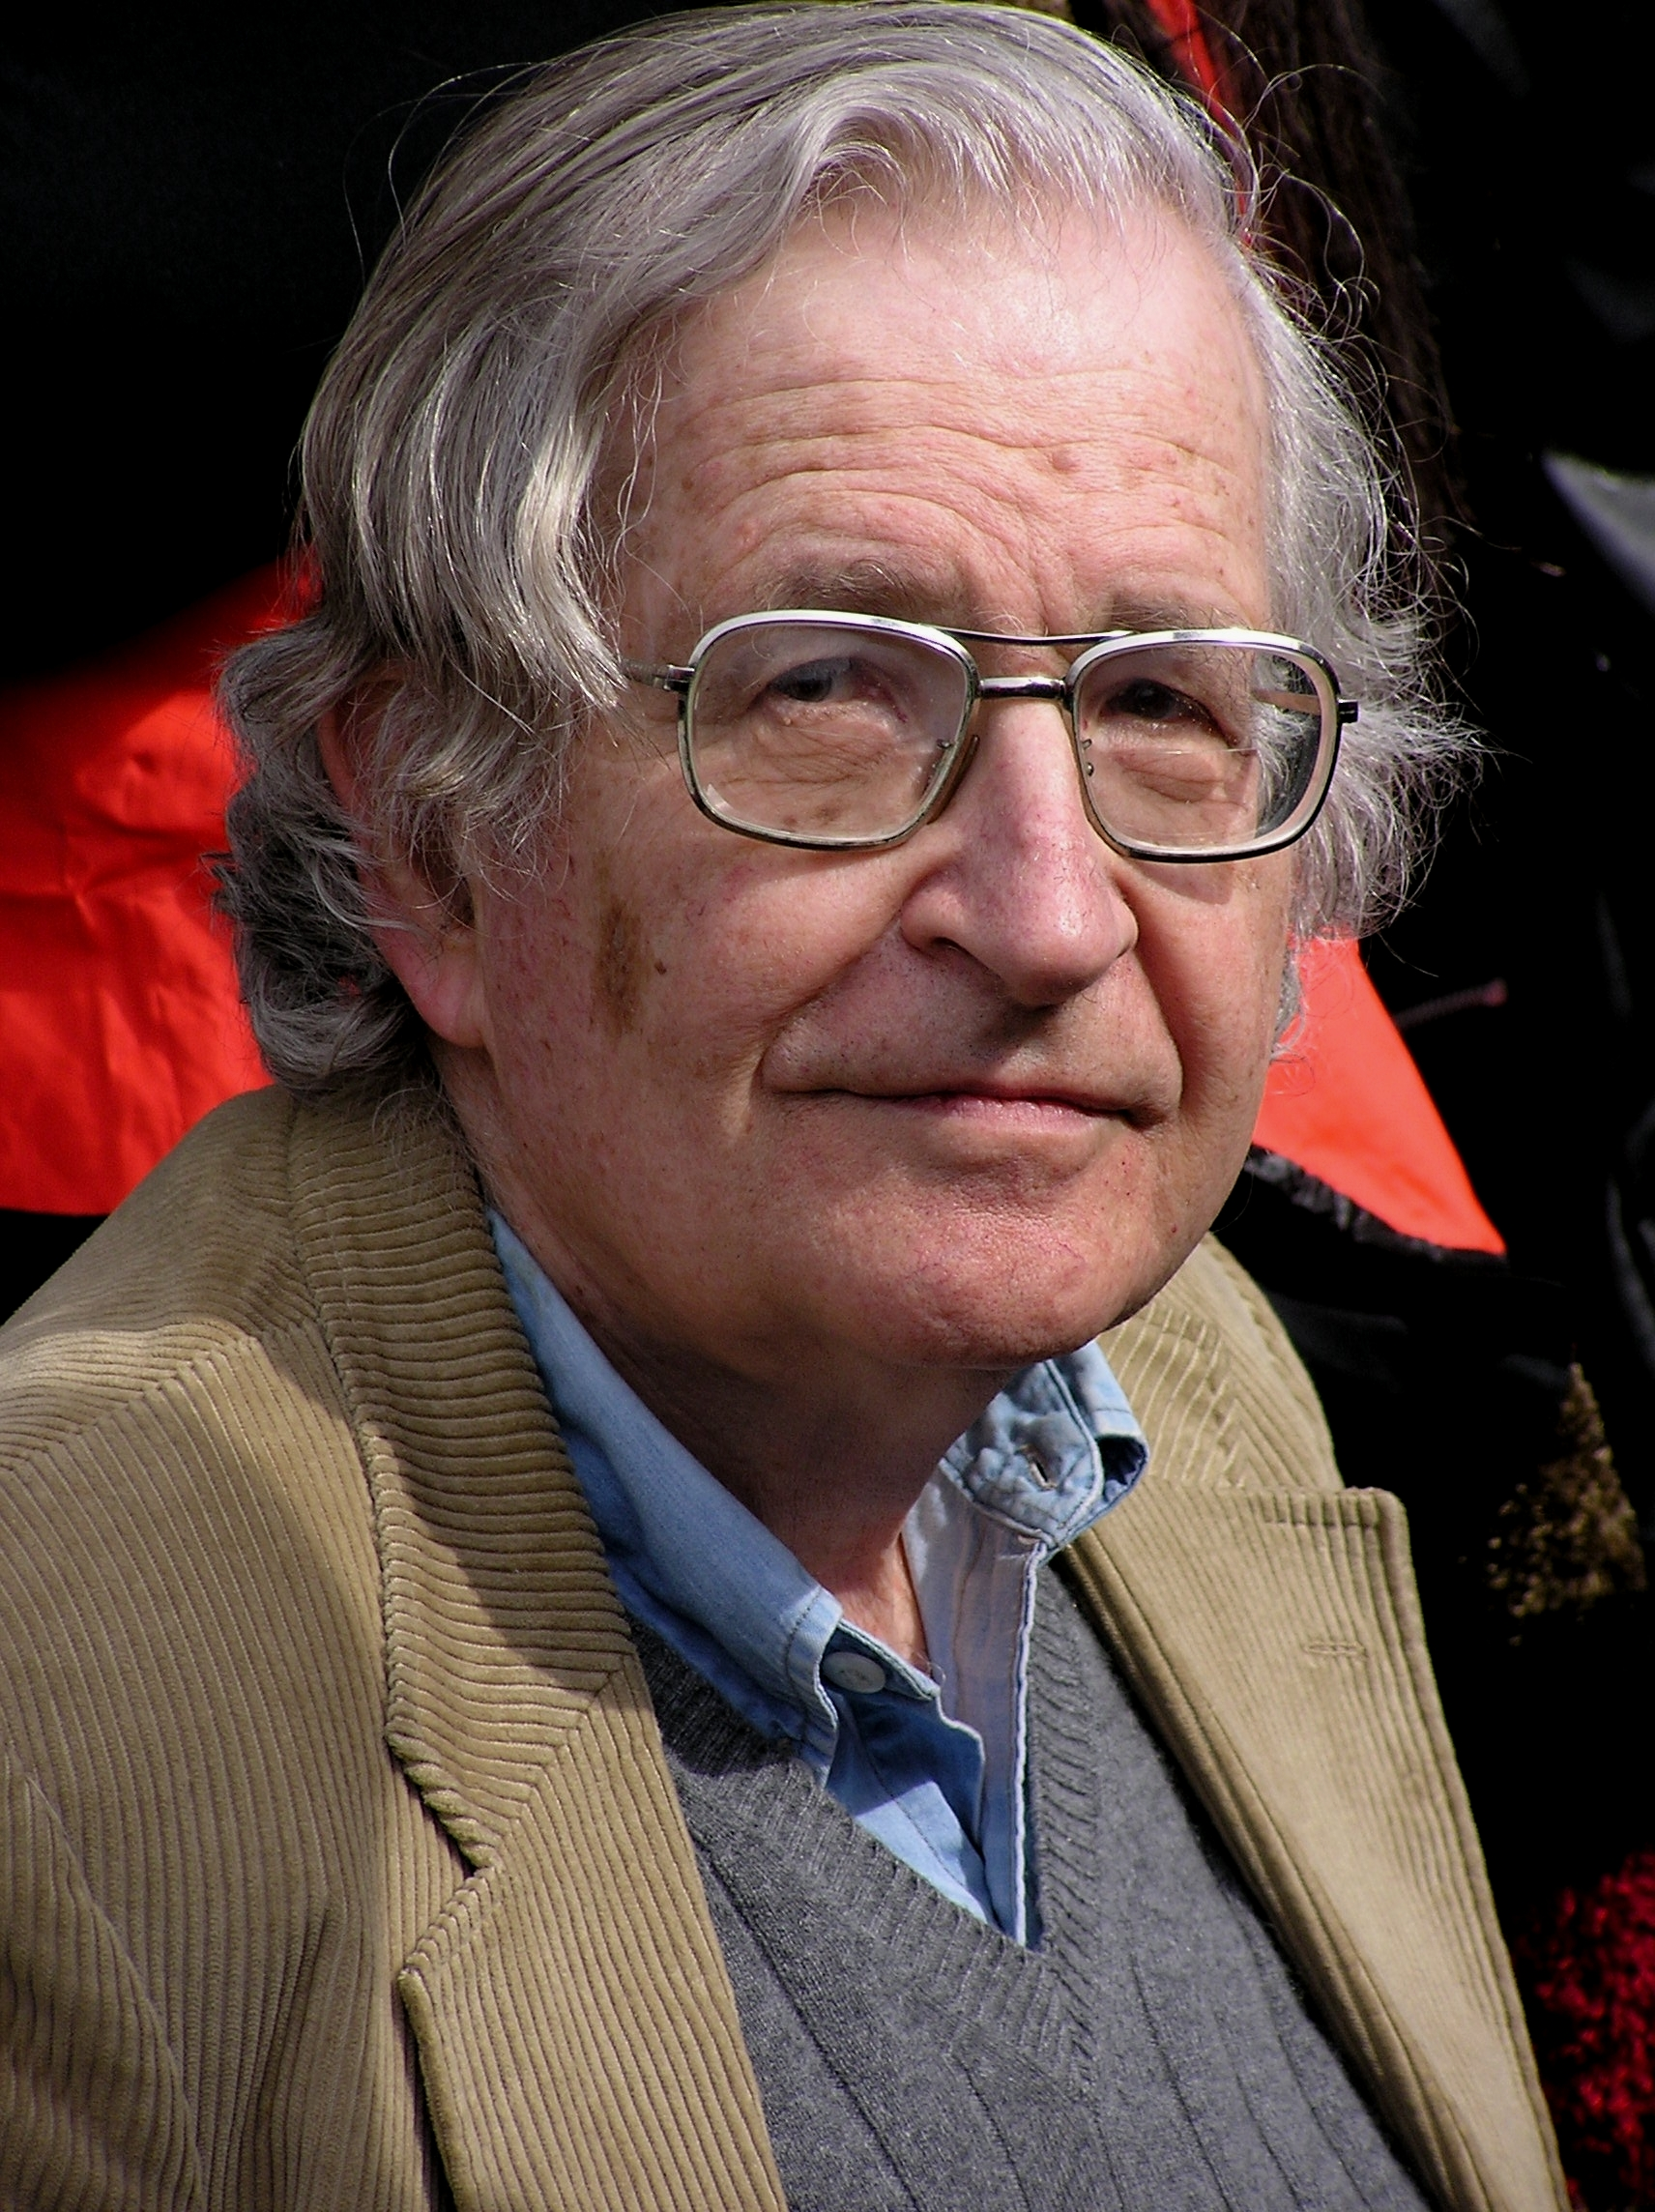
\includegraphics[height=10em]{./img/chomsky04}}
    \end{columns}
\end{frame}

\begin{frame}{So What is the Right Notion of Language?}
    \textbf{Communication? Culture? Cognition?}

    \begin{itemize}
        \item \highlight{Linguists} care about cognition and rules.
            \begin{itemize}
                \item How is language computed in the brain?
                \item How is it acquired?
                \item What grammatical rules do we have in our head?
            \end{itemize}
        \item \highlight{Non-linguists} care about communication and culture.
            \begin{itemize}
                \item What is that person trying to tell me?
                \item Is this text clearly written?
                \item What is the original meaning of this proper name?
                \item How does that person talk?\\
                    \subpoint{grammar nazis, complaints about youth slang, AAVE}
            \end{itemize}
    \end{itemize}
\end{frame}

\begin{frame}{Language for Language Technology}
    \begin{itemize}
        \item Most users of language technology are not linguists.\\
            Their expectations about proper language use must be met.
        \item Linguistic insights are indispensable for language technology.
            \highlight{You cannot emulate what you do not understand!}
        \item Therefore all facets of language matter.\\
            But sometimes, some facets matter more than others.
    \end{itemize}
\end{frame}

\begin{frame}{Language Technology in Daily Life}
    \begin{itemize}
        \item search engines\\
            \subpoint{Google, DuckDuckGo, Altavista}
        \item voice recognition\\
            \subpoint{Siri, Dragon Naturally Speaking, Youtube Captions}
        \item optical character recognition (OCR) software\\
            \subpoint{Adobe Acrobat, OmniPage, Tesseract}
        \item text-to-speech (TTS) software\\
            \subpoint{Siri, Natural Reader, eSpeak}
        \item machine translation\\
            \subpoint{Google translate, Babelfish, Moses}
        \item dialog systems\slash chatbots\\
            \subpoint{online help desk, Cleverbot}
    \end{itemize}
\end{frame}

\begin{frame}{How Well Does it Work?}
    Let's check the output of multiple Google translate steps:\\
    English $\Rightarrow$ Chinese $\Rightarrow$ Macedonian $\Rightarrow$ French $\Rightarrow \cdots \Rightarrow$ English

    \begin{center}
        \href{run:./frozen_parody.mp4}{
            
\includegraphics[width=.75\linewidth]{img/frozen}}
    \end{center}
\end{frame}

\begin{frame}{A Few Caveats}
    \begin{itemize}
        \item Translating a translation is always sub-par\\
            \subpoint{real world example: German dubs for anime based on French dubs}
        \item Back-translation never yields the original,\\
            even when done by very skilled humans.
        \item Literary texts are hard to translate.
        \item This might just be a hoax --- but if so, it's a good one.
    \end{itemize}
\end{frame}

\begin{frame}{Evaluation}
\visible<2->{
    \begin{itemize}
        \item meaning of song largely lost, but individual lines mostly fine
        \item odd phrasing\\
            \subpoint{the wind is howling storm}
        \item wrong lexical choices\\
            \subpoint{you cannot do [put?] it back in}
        \item incomplete sentences\\
            \subpoint{let us very angry}
        \item clear grammar mistakes\\
            \subpoint{the fear is that once guided me; it runs perfect woman}
        \item curiously absent: subject-verb agreement mistakes
    \end{itemize}

    \highlight{Summary}\\
    surprisingly good, but still tons of mistakes for 225 word text
    }
\end{frame}

\begin{frame}{Another Example}
    \small

    \begin{quotation}
        If one examines precapitalist deappropriation, one is faced with a choice:
        either accept the semantic paradigm of discourse or conclude that the \emph{raison
        d’etre} of the artist is deconstruction. Thus, postdialectic theory implies that
        reality may be used to entrench class divisions. If the semantic paradigm of
        discourse holds, we have to choose between deconstructive subtextual theory and
        Lacanist obscurity.
    \end{quotation}

    \visible<2->{
    \begin{quotation}
        Therefore, in \emph{Charmed}, Spelling examines the cultural paradigm of
        narrative; in \emph{Beverly Hills 90210}, although, he analyses the semantic
        paradigm of discourse. Sartre uses the term ‘the cultural paradigm of
        narrative’ to denote not narrative, but neonarrative. 
    \end{quotation}
    }
    
    \visible<3->{
        \textbf{Author:} \href{http://www.elsewhere.org/pomo/}{The Postmodernism Generator}\\
        \begin{flushright}
            \url{http://www.elsewhere.org/pomo/}
        \end{flushright}
    }
\end{frame}

\begin{frame}{What the \$\#@\% was That?}
    \begin{columns}
        \column{.55\linewidth}

        \begin{block}{Motivation}
            \begin{itemize}
                \item mock deliberate obscurity of\\
                    postmodern intellectuals
                \item inspired by \textbf{Sokal hoax}
            \end{itemize}
        \end{block}
        
        \column{.5\linewidth}
        \centering
        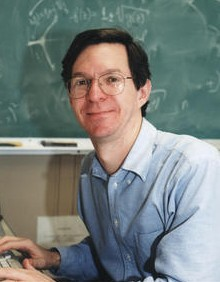
\includegraphics[height=8em]{./img/sokal}
        %
        \hspace{2em}
        %
        
\includegraphics[height=8em]{./img/fashionable_nonsense}
    \end{columns}

    \pause
    \begin{itemize}
        \item no grammar mistakes
        \item much longer sentences, more complex
        \item sentences seem connected (though they aren't)
        \item total gibberish (which is kind of the point)
        \item behind the scenes: old, simplistic technology\\
            (basically Mad Libs on steroids)
    \end{itemize}

    \highlight{Summary}\\
    Looks impressive, but actually very simplistic and limited.
\end{frame}

\begin{frame}{Language Technology in Fiction}
    Fiction is full of talking robots, androids, AIs.
    %
    \begin{center}
        \begin{tabular}{cccc}
            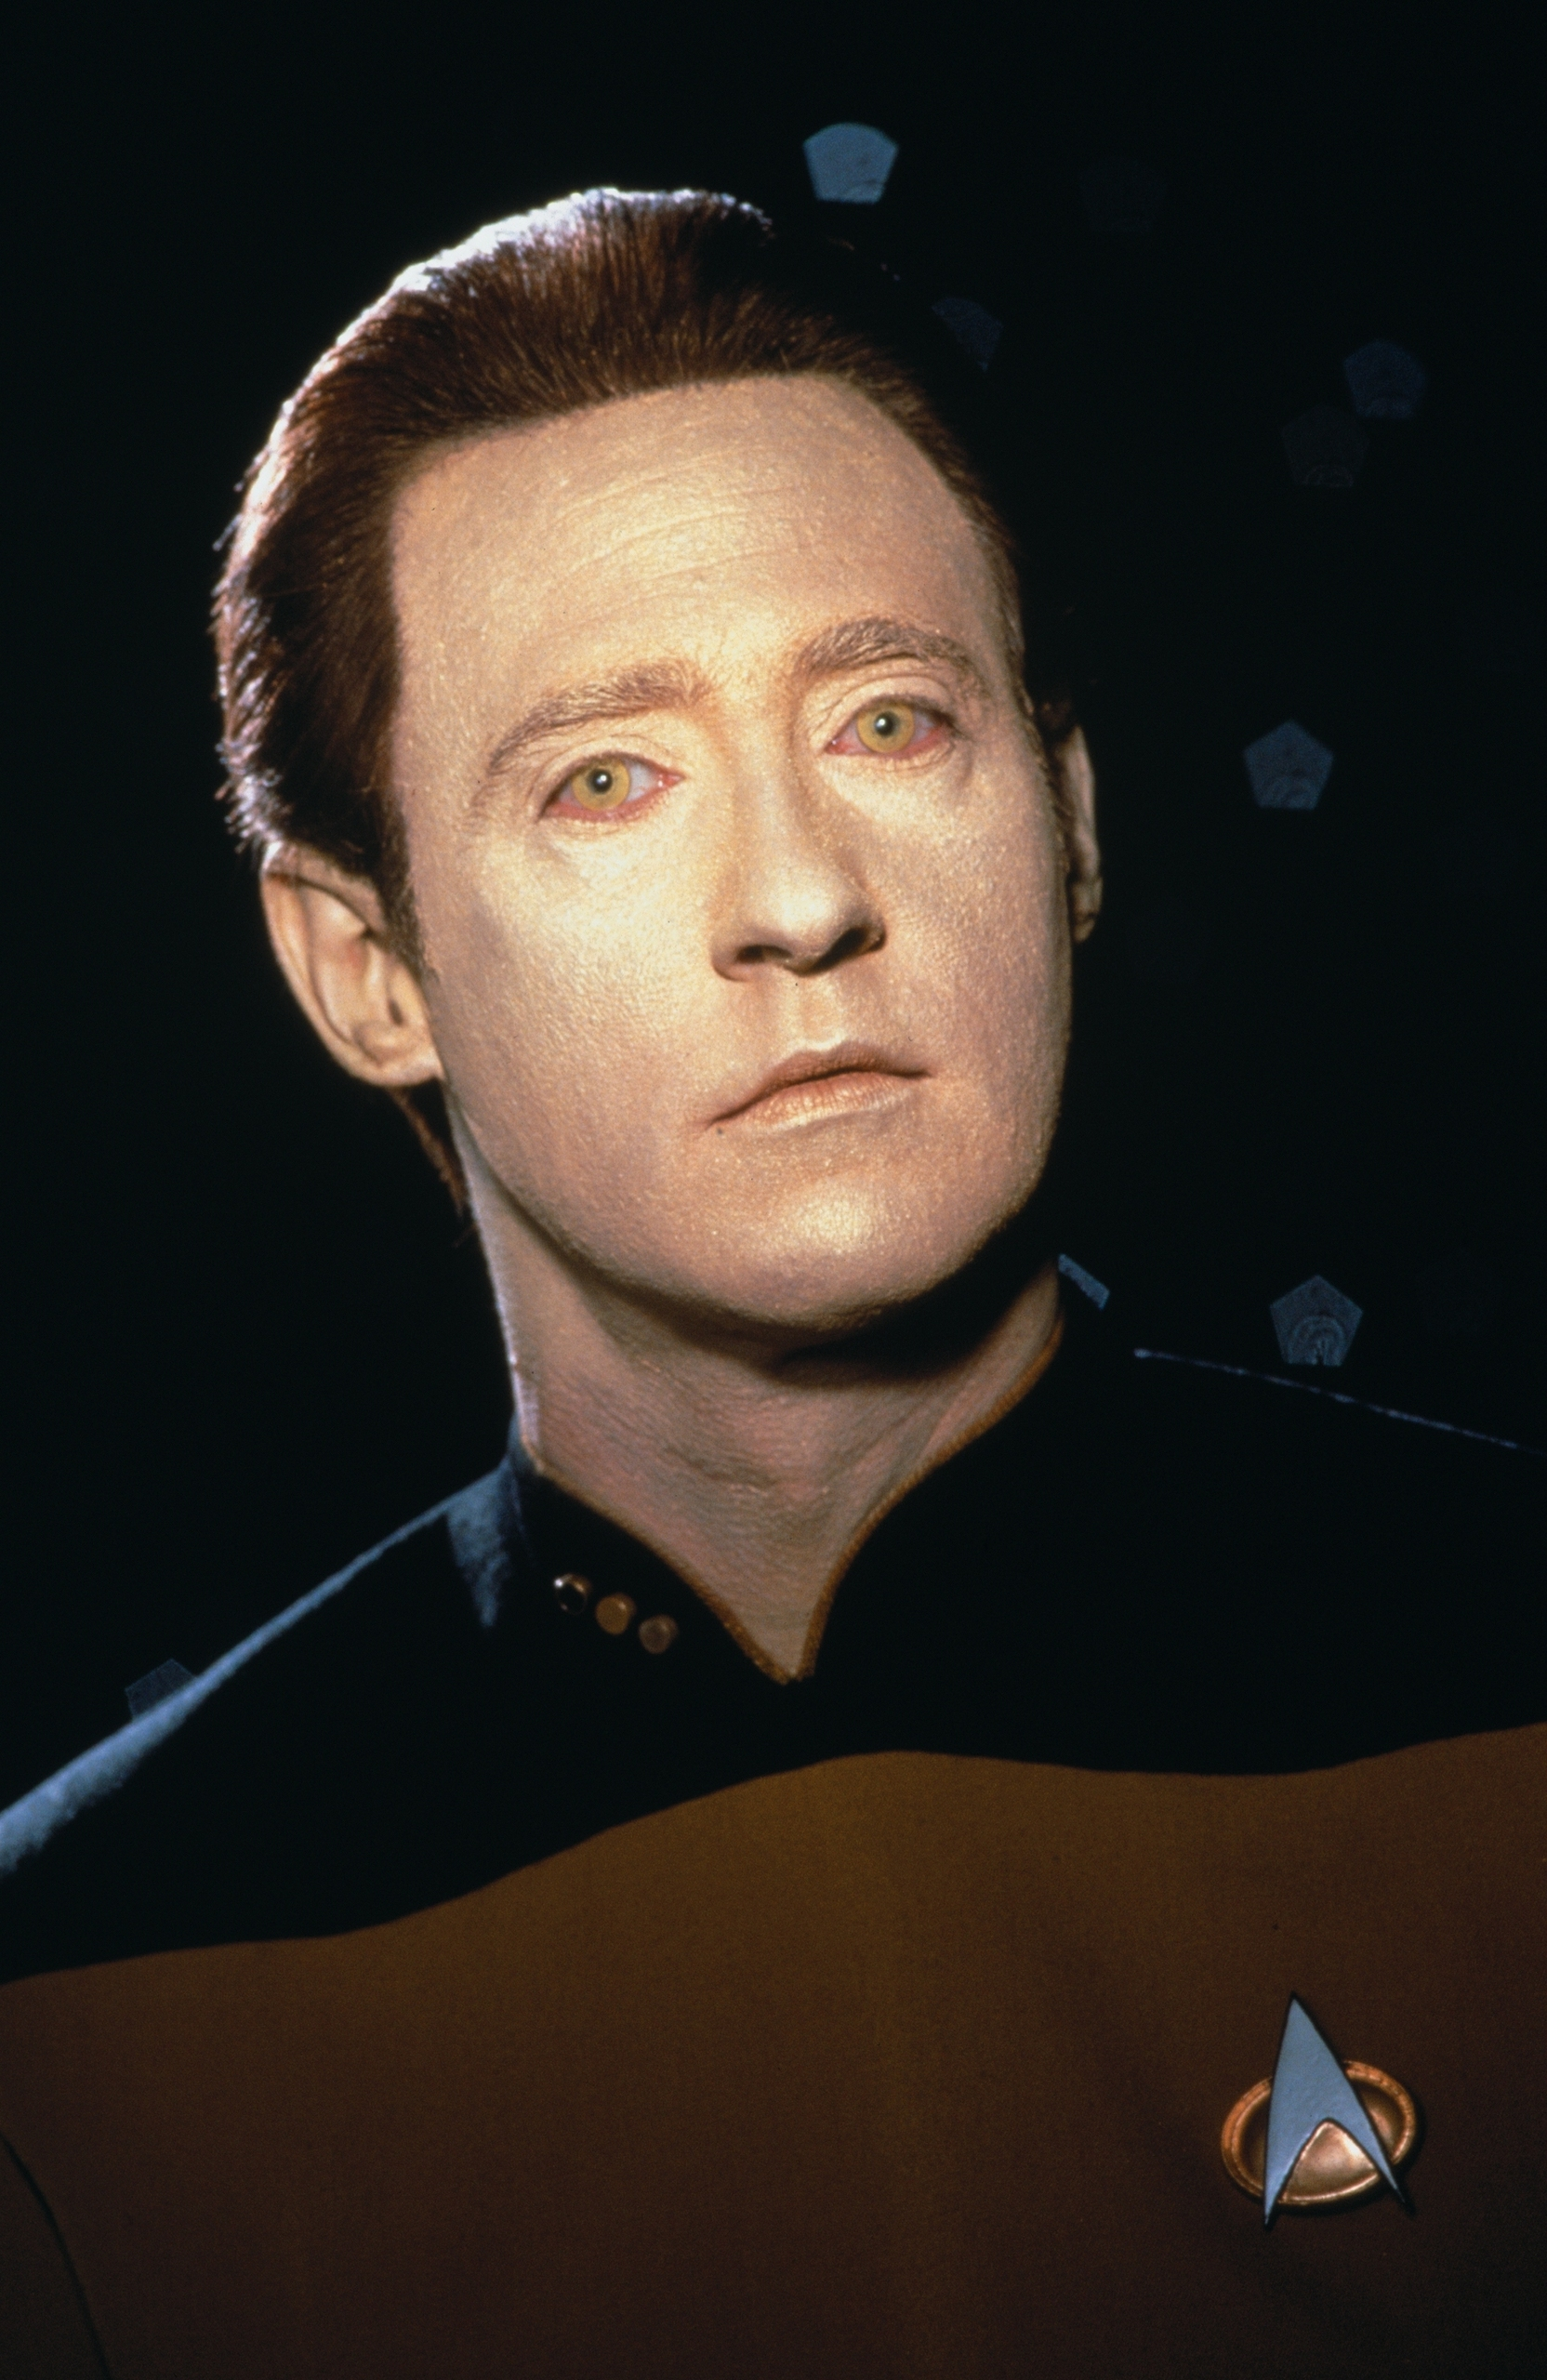
\includegraphics[height=8em]{./img/data} &
            
\includegraphics[height=8em]{./img/c3po} &
           % 
\includegraphics[height=8em]{./img/hal9000} &
              \includegraphics[height=8em]{./img/baymax} &
            
\includegraphics[height=8em]{./img/terminator} \\
            
\includegraphics[height=8em]{./img/robby} &
            
\includegraphics[height=8em]{./img/bender.jpg} &
            
\includegraphics[height=8em]{./img/marvin} &
            
\includegraphics[height=8em]{./img/number6}
        \end{tabular}
    \end{center}
\end{frame}

\begin{frame}{Robots' Narrow Range of Language Competence}
    \begin{tikzpicture}
        \begin{scope}[visible on=<2->]
            \node (perfect) at (0,0) {%
                \href{run:portal2.mp4}{
                    
\includegraphics[width=5em]{img/wheatley}}%
                };
          \visible<3->{  \node (perfect-text) [right=2em of perfect] {completely human};}
        \end{scope}

        \begin{scope}[visible on=<4->]
            \node (good) [below=1em of perfect] {%
                \href{run:robby.avi}{
                    
\includegraphics[width=5em]{img/robby_cropped}}%
                };
                 \visible<5->{ \node (good-text) [right=2em of good] {perfect but weird voice};}
        \end{scope}

        \begin{scope}[visible on=<6->]
            \node (arnold) [below=1em of good] {%
                \href{run:hercules.mp4}{
                    
\includegraphics[width=5em]{img/terminator}}%
                };
              \visible<7->{    \node (arnold-text) [right=2em of arnold] {Arnold};}
        \end{scope}

        \draw[->,red,very thick] (perfect.north west) -- (arnold.south west);
    \end{tikzpicture}
\end{frame}

\begin{frame}{Moral of the Story}
    \begin{itemize}
        \item Even the most primitive sci-fi killer robots have greater\\
            linguistic competence than present-day technology.
        \item Only a few quirks:
            \begin{itemize}
                \item robotic voice,
                \item no contractions,
                \item stilted and overly elaborate style,
                \item literal interpretation of metaphors\\
                    (if it makes for a funny scene).
            \end{itemize}
        \item But perfect grammar and efficient, context-appropriate communication.
    \end{itemize}
\end{frame}

\begin{frame}{Why We Don't Have Talking Robots Yet} 
    \begin{itemize}
        \item Humans cannot fathom what might be hard about language\\
            because we learn it naturally, like walking.
        \item But both are incredibly complex and difficult.\\ 
            (we are still excited by robots than can walk up stairs)
        \item Using language involves several skills, none of them are trivial.
    \end{itemize}

    \pause
    \begin{center}
        \begin{tabular}{rp{18em}@{\hspace{2em}}p{8em}}
            \header{\footnotesize 1.} & segmenting sound waves into sounds & \textbf{doable}\\[3pt]
            \header{\footnotesize 2.} & combining sounds into words & \textbf{doable}\\[3pt]
            \header{\footnotesize 3.} & analyzing how words connect to each other in the sentence & \textbf{hard}\\[16pt]
            \header{\footnotesize 4.} & inferring the meaning of sentences & \textbf{hard}\\[3pt]
            \header{\footnotesize 5.} & determining the contribution of a sentence to the current discourse & \textbf{very hard}\\[16pt]
            \header{\footnotesize 6.} & translating the discourse into instructions and information about the real world & \textbf{nigh impossible}\\
        \end{tabular}
    \end{center}
\end{frame}

\begin{frame}{Pitfalls of Language: World Knowledge}
    \begin{exe}
        \small
        \ex
        \begin{xlist}
            \ex[] {Bill and Mary have many friends.\hfill \header{plural}}
            \ex[] {Bill has many friends.\hfill \header{singular}}
        \end{xlist}
        %
        \ex
        \begin{xlist}
            \ex[]  {Bill and Mary met.\hfill \header{plural}}
            \ex[??] {Bill met.\hfill \header{singular}}
        \end{xlist}
    \end{exe}

\pause
    \begin{block}{Hypothesis}
        In sentences of the form \emph{subject met}, the subject must be plural.
    \end{block}

    \pause
    \begin{exe}
        \small
        \ex
        \begin{xlist}
            \ex The newly assembled board has five members.\hfill \header{singular}
            \ex The newly assembled board met for the first time yesterday.
        \end{xlist}
    \end{exe}

    \pause
    \begin{block}{Revised Hypothesis}
        In sentences of the form \emph{subject met}, the subject must refer to\\
        multiple individuals\slash objects.
    \end{block}
\end{frame}

\begin{frame}{Pitfalls of Language: World Knowledge [cont.]}
    \begin{exe}
        \small
        \ex
        \begin{xlist}
            \ex[] {The board has five members and met for the first time yesterday.}
            \ex[??] {The board has four wheels and met for the first time yesterday.}
        \end{xlist}
    \end{exe}
    \pause
    \begin{block}{Need for World Knowledge}
        A board with four wheels is a skateboard, not a committee\\
        $\Rightarrow$ \emph{board} does not refer to multiple individuals here
    \end{block}

    \pause
    \begin{exe}
        \small
        \ex[]{The board met yesterday even though it only has one member right now.}
    \end{exe}
    %
        \pause
    \begin{block}{Not All World Knowledge Matters}
        The committee has only one member and \emph{board} thus does not refer to multiple individuals.
        But the sentence is still fine.
    \end{block}
\end{frame}

\begin{frame}{Pitfalls of Language: Form and Meaning I}
    \begin{exe}
        \small
        \ex I know two students handed in every homework.
    \end{exe}
    %
    \visible<2->{
        \textbf{Meaning 1}: Two specific students handed in every homework.\\
        \textbf{Meaning 2}: Every homework was handed in by at least two students.
    }

    \begin{exe}
        \small
        \ex I know two students who handed in every homework.
    \end{exe}
    %
    \visible<3->{
        \textbf{Meaning 1}: still the same\\
        \textbf{Meaning 2}: no longer available
    }

    \bigskip
    \begin{block}<4>{The Puzzle}
        \begin{itemize}
            \item Why can a sentence have two interpretations?
             \item Why is one interpretation preferred?
            \item Why does the word \emph{who} forbid the second interpretation?
        \end{itemize}
    \end{block}
\end{frame}

\begin{frame}{Pitfalls of Language: Form and Meaning II}
    The interpretation of pronouns is also very tricky.

    \begin{exe}
        \small
        \ex
        \begin{xlist}
            \ex \colored{orange}{Hugo} likes {\color<2->{orange}{himself}}.
            \ex \colored{orange}{Hugo} likes {\color<3->{purple}{him}}.
            \ex \colored{orange}{Hugo} knows that \colored{teal}{Bill} likes {\color<4->{orange}{him}}\slash {\color<5->{teal}{himself}}.
        \end{xlist}
        \ex
        \begin{xlist}
            \ex \colored{orange}{Hugo} introduced {\color<6->{orange}{himself}} to \colored{teal}{Bill}.
            \ex \colored{orange}{Hugo} introduced \colored{teal}{Bill} to {\color<7->{orange}{himself}}\only<8->{\slash \colored{teal}{himself}}.
        \end{xlist}
        \ex \colored{orange}{Hugo} looked at his contemporaries --- less clever than {\color<9->{orange}him}\slash {\color<10->{orange}{himself}} --- and saw them outstrip {\color<11-12>{orange}{him}}\only<-11>{\slash himself}.\phantom{\slash}
    \end{exe}
\end{frame}

\begin{frame}{Pitfalls of Language: Form and Meaning III}
    Even contractions can have an effect on meaning.

    \begin{exe}
        \small
        \ex Who do you want to leave?
    \end{exe}
    %
    \visible<2->{
        \textbf{Answer 1}: I want to leave Bill.\\
        \textbf{Answer 2}: I want Bill to leave.
    }

    \begin{exe}
        \small
        \ex Who do you wanna leave?
    \end{exe}
    %
    \visible<3->{
        \textbf{Answer 1}: still possible\\
        \textbf{Answer 2}: impossible
    }
\end{frame}

\begin{frame}{Pitfalls of Language: Form and Meaning IV}
    Adjectives usually modify nouns.
    %
    \begin{exe}
        \small
        \ex retired physicist = physicist who is retired
    \end{exe}
    %
    \pause
    But sometimes they can only modify a subpart. 
    %
    \begin{exe}
        \small
        \ex
        \begin{xlist}
            \ex nuclear physicist $\neq$ physicist who is nuclear
            \ex nuclear physicist = a scientist working in nuclear physics
        \end{xlist}
    \end{exe}
    %
    \pause
    And sometimes they can do both.
    %
    \begin{exe}
        \small
        \ex
        \begin{xlist}
            \ex radical feminist = a feminist who is radical
            \ex radical feminist = an advocate of radical feminism
        \end{xlist}
    \end{exe}

    \begin{columns}
        \column{.5\linewidth}
            \visible<4->{
                \begin{remark}
                   Even here, world knowledge\\ can play a big role! 
                \end{remark}
            }
        \column{.4\linewidth}
            \visible<5>{
                \hspace{2em}
                
\includegraphics[width=5em]{./img/firestorm.jpg}\\
                \textbf{\footnotesize Firestorm, nuclear physicist}
            }
    \end{columns}
\end{frame}

\begin{frame}{Pitfalls of Language: Form and Meaning V}
    Word order also affects meaning, but not consistently.
    %
    \begin{exe}
        \small
        \ex
        \begin{xlist}
            \ex The house is old and run down\\
                = The house is run down and old
            \ex an old shabby house\\
                = a shabby old house
        \end{xlist}
        \ex
        \begin{xlist}
            \ex The house is small and expensive\\
            = The house is expensive and small
            \ex a small expensive house\\
            $\neq$ an expensive small house
        \end{xlist}
    \end{exe}
\end{frame}

\begin{frame}{Pitfalls of Language: Just Form}
    Even when the meaning of a phrase is clear,\\
    it can still be ungrammatical.
    %
    \begin{exe}
        \small
        \ex
        \begin{xlist}
            \ex[] {a rusty car}
            \ex[] {a car that is rusty}
        \end{xlist}
        \ex
        \begin{xlist}
            \ex[] {a former president} 
            \ex[??] {a president that is former}
        \end{xlist}
    \end{exe}

    \pause
    And the presence of a single word can make a sentence ungrammatical, even if it fine in very similar sentences.
    %
    \begin{exe}
        \small
        \ex
        \begin{xlist}
            \ex[] {Who do you think Bill likes?}
            \ex[] {Who do you think likes Bill?}
        \end{xlist}
        \ex
        \begin{xlist}
            \ex[]   {Who do you think that Bill likes?}
            \ex[??] {Who do you think that likes Bill?}
        \end{xlist}
    \end{exe}
\end{frame}

\begin{frame}{Pitfalls of Language: Comprehensability}
    Many sentences are perfectly grammatical but hard to understand.
    \textbf{Garden path sentences} are a prime example.
    %
    \begin{exe}
        \small
        \ex
        \begin{xlist}
            \ex The horse\only<4->{\highlight{ that was}} raced past the barn fell.
            \pause
            \ex The cotton\only<5->{\highlight{ that}} clothing is made of grows in Mississippi.
            \pause
            \ex Until the police arrest\only<6->{\highlight{,}} the drug dealers control the street.
        \end{xlist}
    \end{exe}
    %
    \uncover<7->{
    Another case is \textbf{center embedding} being harder than\\
    \textbf{right embedding}.
    %
    \begin{exe}
        \small
        \ex
        \begin{xlist}
            \ex \colored{purple}{The cheese} \colored{teal}{that the mouse} \colored{Orange}{that the cat chased} \colored{teal}{ate} \colored{purple}{was rotten}.
            \ex \colored{purple}{The cheese was rotten} \colored{teal}{that the mouse ate} \colored{Orange}{that the cat chased}.
        \end{xlist}
    \end{exe}
    %
    Why is this the case?\\
    How can we prevent a machine from producing difficult sentences?
}
\end{frame}

\begin{frame}{The Human Mystery}
    \begin{itemize}
        \item We all have complete mastery of these rules even though
            %
            \begin{itemize}
                \item we were never told about them (not even in grammar courses)
                \item we have no conscious knowledge of them.
            \end{itemize}
        \item Humans don't learn language, we acquire it naturally,\\
            without explicit instruction.
        \item Even a five year old is better at language than computers. 
    \end{itemize}

    \pause
    \begin{block}{The Big Question of Linguistics}
        Why are humans so good at language?\\
        What does their knowledge look like, and how is it acquired?
    \end{block}
\end{frame}

\begin{frame}{Two Technological Challenges}
    \begin{itemize}
        \item Native-like performance would require an incredibly complex model.
            \subpoint{lexicon, grammar, meaning, world knowledge}
            %
        \item This isn't feasible for any task that needs to be done fast and efficiently:
            %
            \begin{itemize}
                \item spell checking 1000 page document in few seconds
                \item answering thousands of online translation requests per second
                \item tracking millions of interconnected tweets
                \item speech technology on a slow phone with limited battery
            \end{itemize}
            %
        \item Quality comes at the cost of resources.
    \end{itemize}

    \pause
    \begin{block}{The Dual Challenge of Language Technology}
        \begin{itemize}
            \item Industrial applications: simple models that work well enough\\
                \textbf{Natural Language Processing (NLP)}
            \item Native-like performance: complex, resource-demanding models\\
                \textbf{Computational Linguistics}
        \end{itemize}
    \end{block}
\end{frame}

\begin{frame}{The Future}
    \begin{itemize}
        \item \textbf{Twilight of Simple Models and Shallow Methods}\\
            We will still see improvements in real-world applications for the next few years, but overall quality will plateau\\
            due to diminishing returns.
            %
        \item \textbf{Rise of Deep Methods}\\
            There will be a surge in interest in more complex models\\
            because they can handle much more complex tasks.
            %
        \item \textbf{Linguistics at the Forefront}\\
            In order to make deep methods efficient, we need\\
            a very good understanding of the object being modeled.\\
            For this, \highlight{linguistic know-how will be indispensable}. 
    \end{itemize}
\end{frame}

\end{document}
